%% This is an example first chapter.  You should put chapter/appendix that you
%% write into a separate file, and add a line \include{yourfilename} to
%% main.tex, where `yourfilename.tex' is the name of the chapter/appendix file.
%% You can process specific files by typing their names in at the 
%% \files=
%% prompt when you run the file main.tex through LaTeX.

\begingroup%
\makeatletter%
\cleardoublepage%
\let\newpage\relax%
\let\clearpage\relax%
\vspace*{\fill}%
\vspace*{\dimexpr-50\p@-\baselineskip}% Remove the initial
%% -default- 50pt gap (plus 1 line) 
\chapter[Supporting information for Chapter 4]{{\setlength{\huge} Supporting information for}\\ \autoref{chap4}: Mechanisms and Biogeochemical Significance of Lipid Photooxidation in Coastal Surface Waters of West Antarctica}
\label{AppE}
\vspace*{\fill}%
\endgroup%

\clearpage

\section{Supplementary Methodological Details Not Described in the Text}

\subsection{Sample Injection, Chromatography and ESI Source Settings}

20 $\mu$L injections of sample were made onto a C8 Xbridge HPLC column (particle size 5 $\mu$m, length 150 mm, width 2.1 mm; Waters Corp., Milford, MA, USA). Eluent A consisted of water with 1\% 1M ammonium acetate and 0.1\% acetic acid. Eluent B consisted of 70\% acetonitrile, 30\% isopropanol with 1\% 1M ammonium acetate and 0.1\% acetic acid. Gradient elution was performed with the following program (total run time 40 min) at a constant flow rate of 0.4 mL min\textsuperscript{-1}: 45\% A for 1 min to 35\% A at 4 min, then from 25\% A to 11\% A at 12 min, then to 1\% A at 15 min with an isocratic hold until 30 min, and finally back to 45\% A for 10 min column equilibration. ESI source settings were: Spray voltage, 4.5kV (+), 3.5 kV (-); capillary temperature, 200$^{\circ}$C; sheath gas and auxiliary gas, both 20 (arbitrary units); heated ESI probe temperature, 350$^{\circ}$C.

\subsection{Mass Spectrometer Acquisition Settings}
\label{ssec:Mass Spectrometer Acquisition Settings}

Mass data were collected on a Thermo Q Exactive Hybrid Quadrupole-Orbitrap mass spectrometer (ThermoFisher Scientific, Waltham, MA, USA) instrument in full scan and TopN data dependent-MS\textsuperscript{2} (dd-MS\textsuperscript{2}) acquisition modes while alternating between positive and negative ionization modes. Following the full spectrum scan in each mode (scan range of 100-1500 \emph{m/z}), the five ions of highest intensity were selected using the quadrupole for MS\textsuperscript{2} fragmentation. Data were acquired in the following sequence: FT positive full lock MS, positive-mode dd-MS\textsuperscript{2}, FT negative full lock MS, and negative-mode dd-MS\textsuperscript{2}. The S-lens RF level and voltage were set to 100.00\% and 25.00 V, respectively. Mass resolution was set to the maximum possible value of 140,000 (FWHM at \emph{m/z} 200) for full scan acquisition and to 17,500 for dd-MS\textsuperscript{2} scans. The full scan mass resolution setting corresponded to an observed resolution of 75,100 at the \emph{m/z} (875.5505) of our internal standard, DNP-PE, in positive ion mode. Using these settings, we obtained between 8 and 14 MS scans across a typical peak in full scan mode. The following other settings were applied: MS\textsuperscript{2} isolation window, 4 \emph{m/z}; MS\textsuperscript{2} isolation offset, 0.00; loop count, 5; dynamic exclusion, 10.0 s; AGC target, 3,000,000/100,000 (full scan/MS\textsuperscript{2}); skimmer voltage, 15.00 V; inject flatapole DC, 6.00; MP2 and MP3 RF, 594; gate lens voltage, 5.88 V; C-trap RF, 1,010; MS\textsuperscript{2} NCE/stepped NCE, 30, 50, 80.

\subsection{Procedures Used for Weekly and Real-Time Calibration of the Exactive}

The mass spectrometer was calibrated as requried in both positive and negative ion modes by infusing calibration mixes available from ThermoFisher Scientific. Deliberate lock masses were also used for real-time recalibration; C\textsubscript{16:0} (\emph{m/z} 255.23295) and C\textsubscript{18:0} (\emph{m/z} 283.26425) fatty acids were used in negative ion mode, while ammonium adducts of a series of polysiloxanes (\emph{m/z} 536.16537, 610.1842, and 684.2035) were used in positive ion mode. At least one of the lock masses was found during each positive and negative full scan event.

\clearpage

\section{Supplementary Figures}

\begin{figure}[!th]
\centering
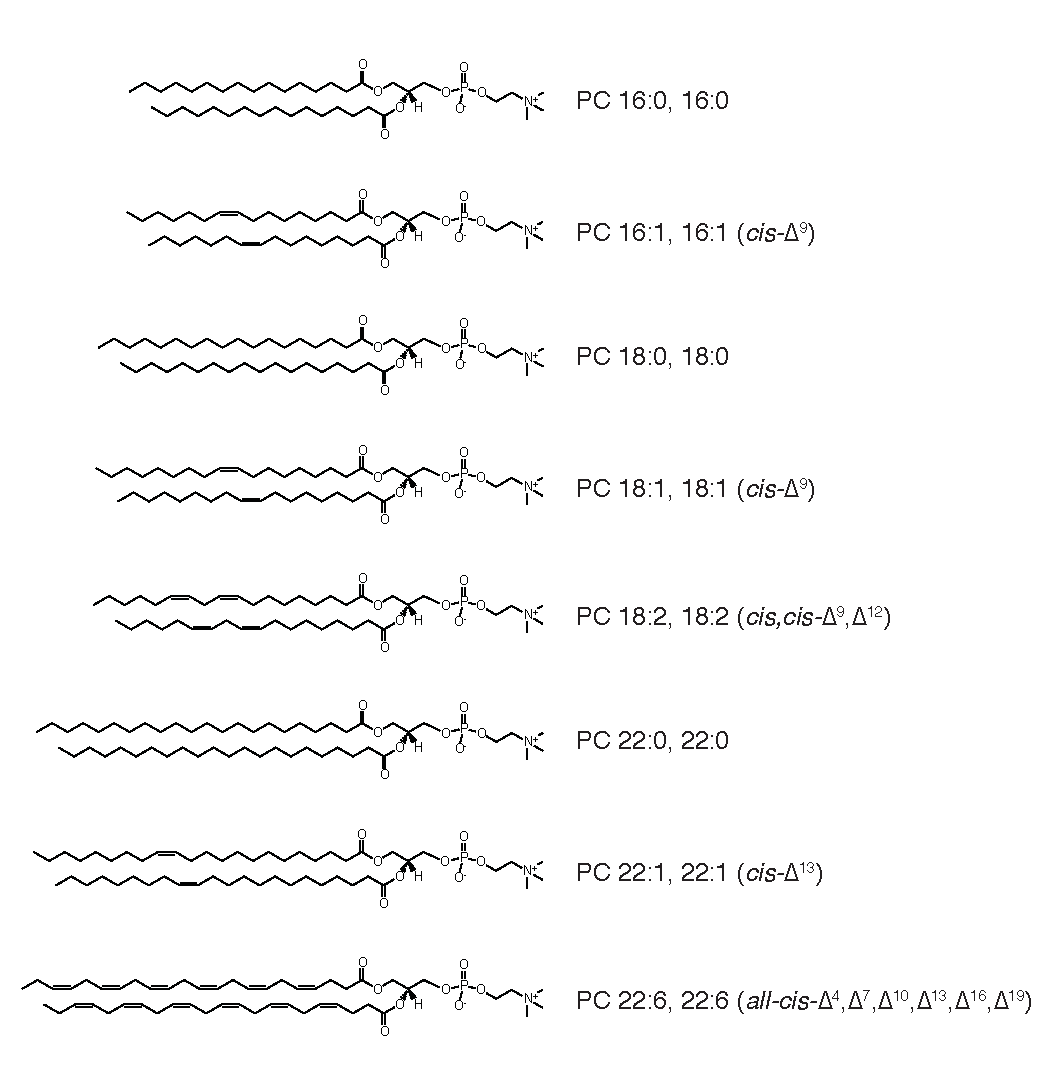
\includegraphics[width=1\textwidth]{Fig_E-1.pdf}
\captionsetup{font={footnotesize}}
\caption[Structures of the eight species of phosphatidylcholine evaluated in photooxidation experiments]{Structures of the eight species of phosphatidylcholine (PC) evaluated in the photooxidation experiments described in the text.}
\label{fig:aen1}
\end{figure}

\clearpage

\begin{figure}[!th]
\centering
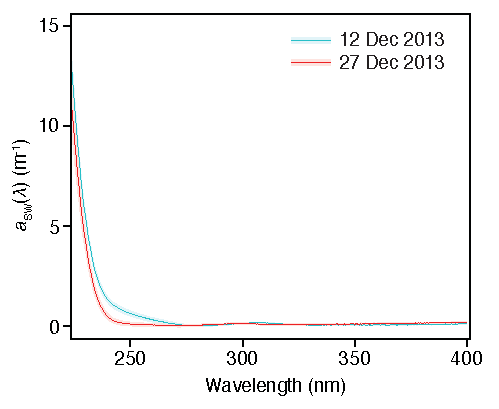
\includegraphics[width=.6\textwidth]{Fig_E-2.pdf}
\captionsetup{font={footnotesize}}
\caption[Wavelength-specific absorbance coefficients of West Antarctic Peninsula surface waters]{Wavelength-specific absorbance coefficients (${a_{SW}}(\lambda )$) of West Antarctic Peninsula surface waters from samples collected on two dates in December 2013. For each date, we report the mean values of ${a_{SW}}(\lambda )$ determined for each wavelength in a set of samples collected at 0, 5, and 10 m. The 27 December values (red trace) reflect samples collected at the three depths at both PAL-LTER time series stations (B and E; \emph{N} = 6), while the 12 December values (blue trace) are based only on samples collected at Station B (\emph{N} = 3). The shaded region surrounding each trace depicts one standard deviation. Values of ${a_{SW}}(\lambda )$ were calculated according to \autoref{eq:c4e4} in the text.}
\label{fig:aen2}
\end{figure}

\clearpage

\begin{figure}[!th]
\centering
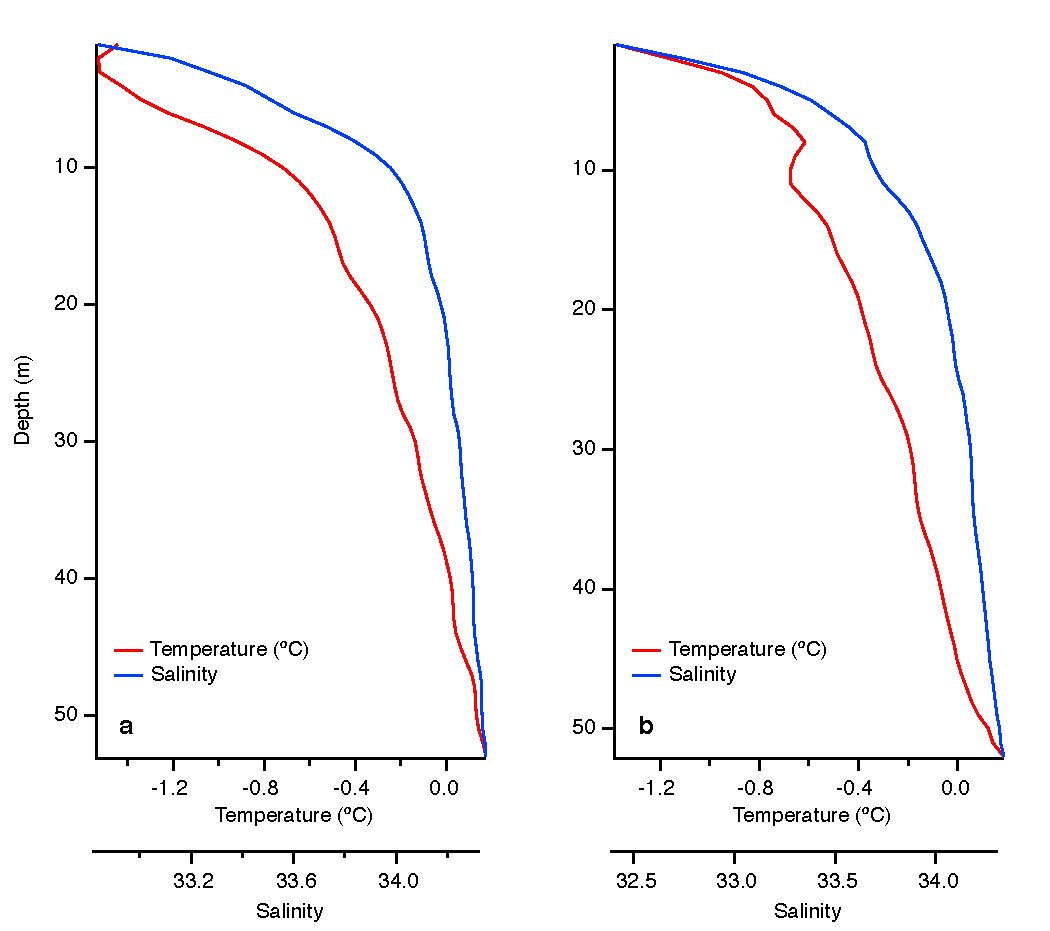
\includegraphics[width=.9\textwidth]{Fig_E-3.pdf}
\captionsetup{font={footnotesize}}
\caption[Profiles of temperature and salinity made at PAL-LTER Station B in December 2013]{Profiles of temperature and salinity made at PAL-LTER Station B on (a) 12 December and (b) 24 December 2013. The data from which these figures were constructed were retrieved from \url{http://oceaninformatics.ucsd.edu/datazoo/data/pallter/datasets?action=summary&id=228} on 1 November 2016. The location of Station B in Arthur Harbor is shown in \autoref{fig:c4n1}.}
\label{fig:aen3}
\end{figure}

\clearpage

\begin{landscape}
\begin{figure}[p]
\vspace*{-1.5cm}
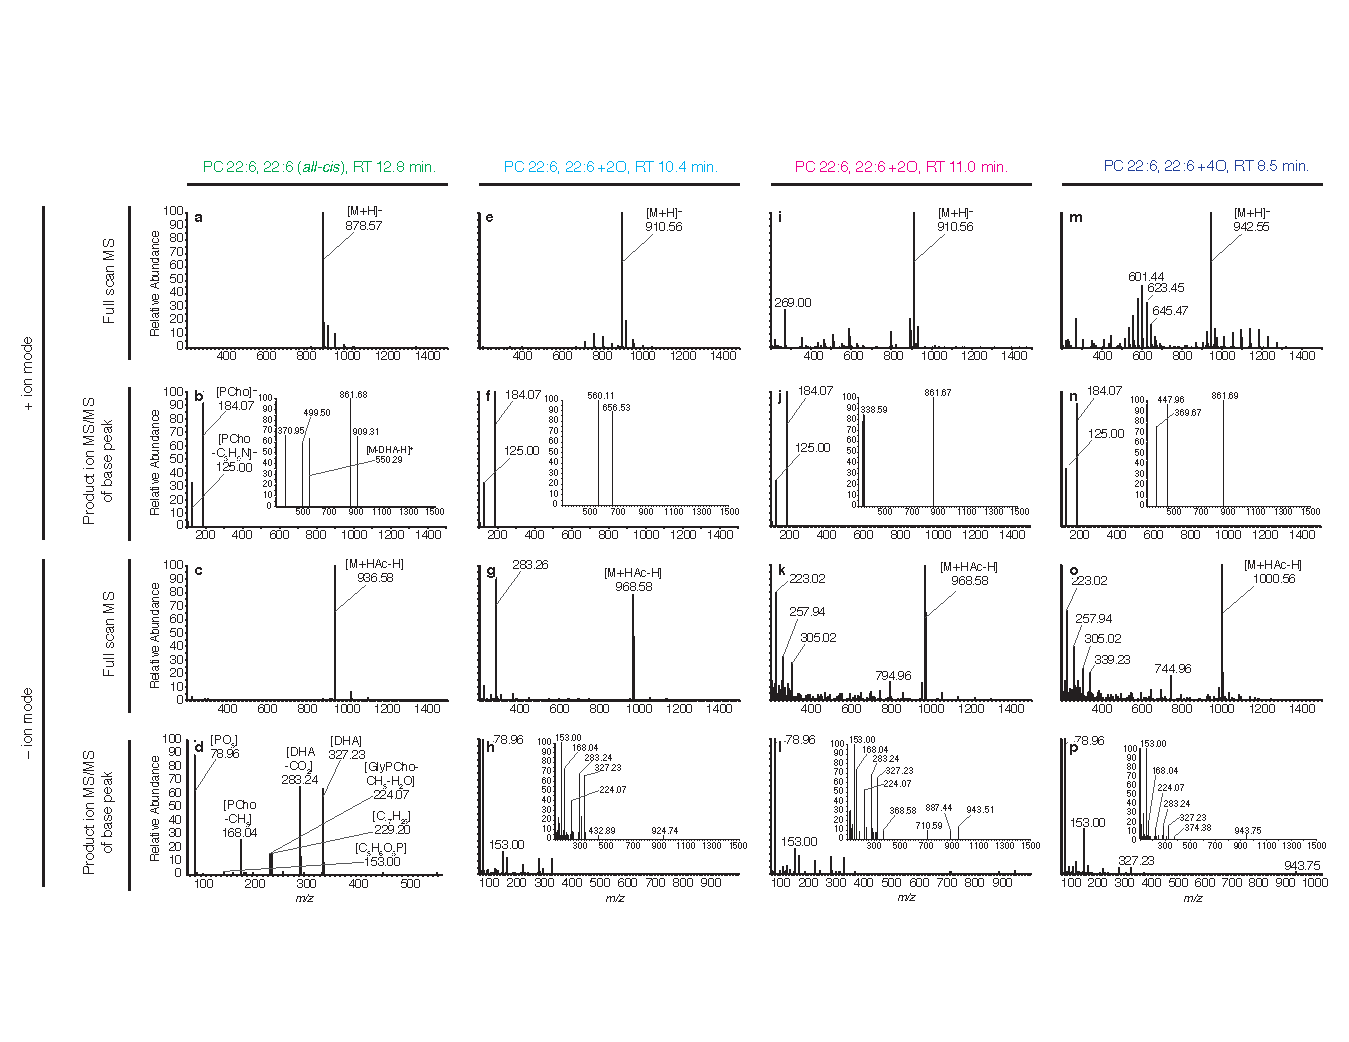
\includegraphics[width=1\linewidth]{Fig_E-4.pdf}
\end{figure}
\clearpage
\end{landscape}
\begingroup
\captionsetup{font={footnotesize}}
\captionof{figure}[Expanded version of \autoref{fig:c4n9}]{(preceding page) Expanded version of \autoref{fig:c4n9} in the main text, showing annotated positive and negative ion mode spectra used to identify three intact oxidized products of PC 22:6, 22:6 (\emph{all-cis}-$\Delta$\textsuperscript{4},$\Delta$\textsuperscript{7},$\Delta$\textsuperscript{10},$\Delta$\textsuperscript{13},$\Delta$\textsuperscript{16},$\Delta$\textsuperscript{19}) in a lipid photooxidation experiment on 14 December 2013. The spectra presented here are from one of three replicate samples of the +UVB --het. bact. treatment at the final experimental time point shown in \autoref{fig:c4n6}. Product ion spectra (second and fourth rows) were obtained via data-dependent MS\textsuperscript{2} using a Thermo Q Exactive Hybrid Quadrupole-Orbitrap mass spectrometer; MS and HPLC conditions are described in the Supporting Information text. Panels (a)-(d) show diagnostic spectra for the intact parent PC 22:6, 22:6 molecule ({[}M+H{]}\textsuperscript{+} and {[}M-HAc-H{]}\textsuperscript{-} adducts, respectively); these were validated by comparison with an authentic standard. Panels (e)-(h), (i)-(l), and (m)-(p) show, respectively, spectra for three ox-PC 22:6. 22:6 species identified at 10.4, 11.0, and 8.5 min. Colors in column headings correspond to those used in \autoref{fig:c4n8} and \autoref{fig:c4n9} in the text. Insets show the relative intensities of ions $\geq$ 300 or 100 \emph{m/z} units (positive and negative ionization modes, respectively). Although we were unable to identify the precise structures of the three ox-PC species without further fragmentation (i.e., MS\textsuperscript{n}; see discussion in text), we offer five lines of evidence for identities of these species as +2O and +4O products of the parent molecule, with the additional conviction that the oxidation in each case oc$\mu$red at a specific position on one of the two attached acyl chains: (1) the knowledge that, by virtue of the experimental design, the observed species must be degradation products of one of the five lipids we added as liposomes, (2) agreement at $\leq$ 0.3 ppm of the exact masses of the parent ion adducts in both ionization modes with calculated theoretical masses, (3) systematic shifts in retention time consistent with the progressive addition of oxygen atoms, (4) the unique fragmentation spectra observed, each containing ions not present in those obtained for the parent molecule, and (5) the presence in all three of the negative ion mode MS\textsuperscript{2} spectra of the \emph{m/z} 327.23, 224.07, and 283.24 fragments diagnostic of the presence of intact, unoxidized DHA.}
\label{fig:aen4}
\endgroup

\clearpage

\begin{figure}[!th]
\centering
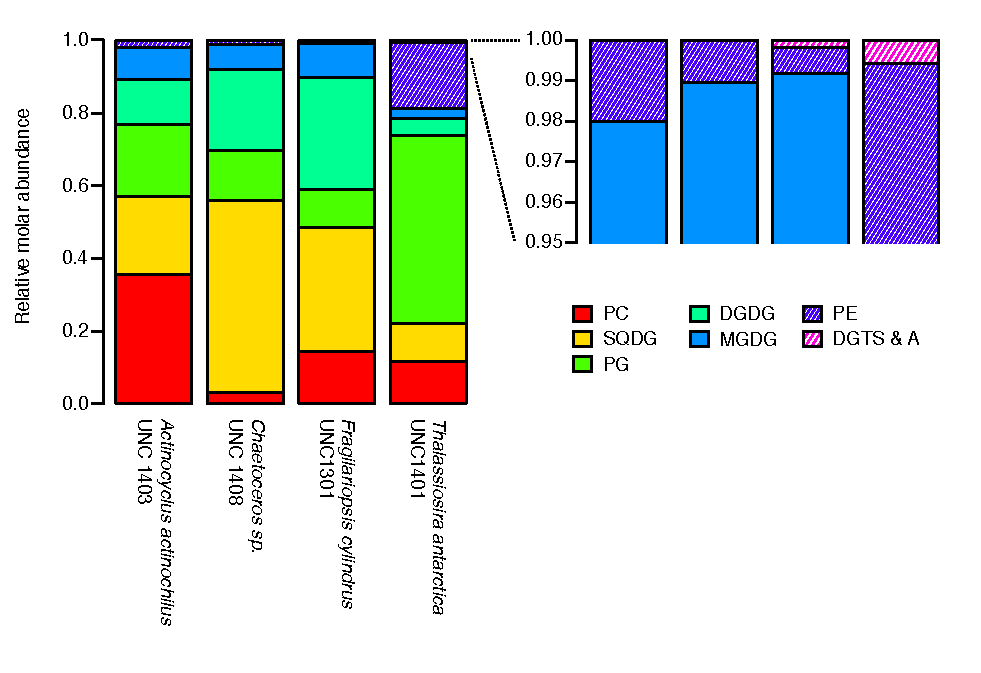
\includegraphics[width=.9\textwidth]{Fig_E-5.pdf}
\captionsetup{font={footnotesize}}
\caption[Relative molar distribution of seven classes of IP-DAG in cultures of four diatom species isolated from waters of the West Antarctic Peninsula]{Relative molar distribution of seven classes of intact polar diacylglycerol (IP-DAG) in cultures of four diatom species isolated from waters of the West Antarctic Peninsula. Cultures were grown in nutrient replete medium and biomass was harvested in exponential growth phase. Lipids were identified using the LOBSTAHS software and several additional criteria described in the main text; the data in this figure represent 316 different IP-DAG identified in the four isolates. Quantification of lipids was performed using authentic standards as described in the main text. We also identified several species of diacylglyceryl carboxyhydroxymethylcholine (DGCC) in the isolates; these were excluded from the dataset used to generate the figure because we did not have a suitable authentic standard available at the time of analysis. DGCC accounted for \textless{} 1 \% of the total raw IP-DAG peak area in \emph{A. actinochilus} and \emph{F. cylindrus}, \textless{} 3 \% in \emph{Chaetoceros sp.}, and $\sim$ 20 \% of the total IP-DAG peak area in \emph{T. antarctica}. The diatom cultures were kindly provided by C. Moreno and A. Marchetti, University of North Carolina. The full, annotated list of the lipids identified in each culture is available online at \url{https://github.com/jamesrco/LipidPhotoOxBox/blob/master/data/nice/LOBSTAHS_lipid_identities/UNC_Marchetti_diatom_cultures_IP-DAG_pmol_totals.final.csv} or upon request from the author.}
\label{fig:aen5}
\end{figure}

\clearpage

\begin{figure}[!th]
\centering
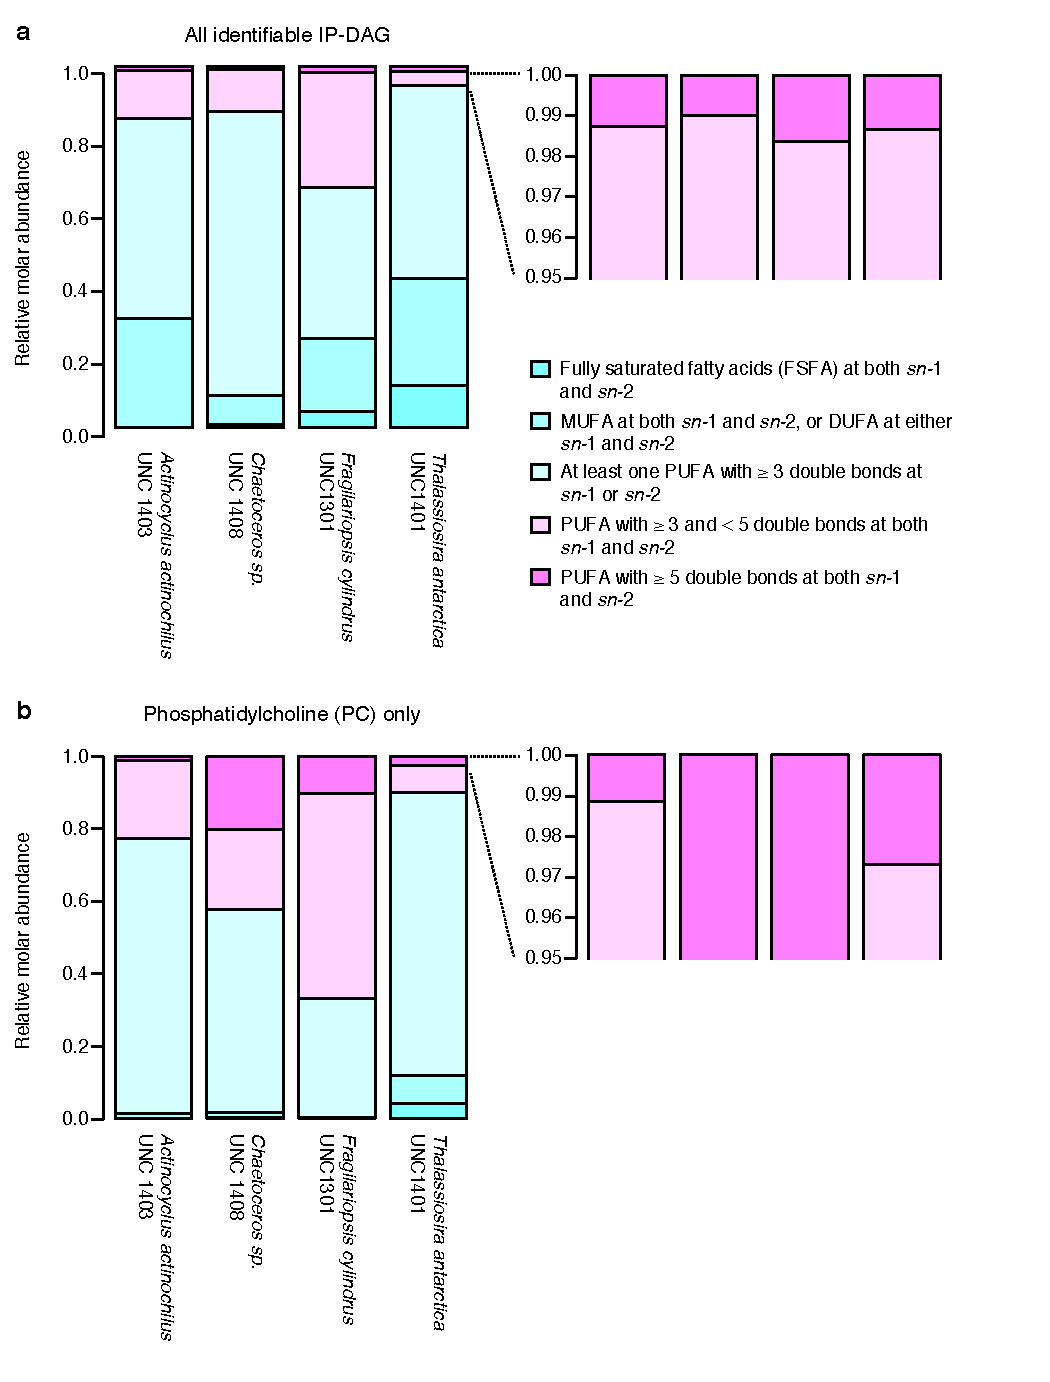
\includegraphics[width=.9\textwidth]{Fig_E-6.pdf}
\captionsetup{font={footnotesize}}
\caption[Fatty acid composition of IP-DAG in the four Antarctic diatom isolates presented in \autoref{fig:aen5}]{Fatty acid composition of (a) all identifiable IP-DAG and (b) phosphatidylcholine (PC) species in the four Antarctic diatom isolates for which distributions of IP-DAG are presented in \autoref{fig:aen5}. Because the current version of the LOBSTAHS software resolves the identities of IP-DAG~only to the level of bulk fatty acid composition (i.e., the sum of the properties of the substituents at both the \emph{sn}-1 and \emph{sn}-2 positions), we were unable to determine which fatty acids were present in each molecule without significant additional inspection of fragmentation spectra or saponification for analysis fatty acid methyl esters (FAMES). We were able to categorize the saturation state of the IP-DAG according to the simplified scheme we present here after verifying (by inspection of fragmentation spectra) that the maximum degree of unsaturation of any single fatty acid present in these species was six (present in the form of docosahexaenoic acid, or DHA).}
\label{fig:aen6}
\end{figure}

\clearpage

\section{Supplementary Tables}

\clearpage

\begin{landscape}

\begin{footnotesize}
\begin{singlespace}
\begin{flushleft}
\begin{longtable}{ Lp{.1\linewidth} Lp{.1\linewidth} Lp{.1\linewidth} Lp{.11\linewidth} Lp{.11\linewidth} Lp{.11\linewidth} Lp{.11\linewidth} Lp{.11\linewidth} }
\captionsetup{font={normalsize}}
\caption[Summary of Results from Liposome Photooxidation Experiments]{Summary of Results from Liposome Photooxidation Experiments}\\
\label{table:aen1}
\endfirsthead
\endhead
\toprule
\multirow{3}{\linewidth}[0em]{Moiety Phosphatidyl-choline} & \multirow{3}{\linewidth}[0em]{No. Independent Experiments in which Evaluated} & \multirow{3}{\linewidth}[0em]{Date of Experiment (2013)} & \multicolumn{5}{ l }{Rate of Change in Concentration\textsuperscript{a} (pmol mL\textsuperscript{-1} hr\textsuperscript{-1} $\pm$ SE)} \\
\cmidrule{4-8}
 &  &  & \multicolumn{5}{ l }{Treatment}  \\
\cmidrule{4-8}
 &  &  & Control (dark) -- het. bact. & Control (dark) + het. bact & -- UVB -- het. bact.\textsuperscript{b} & + UVB -- het. bact.\textsuperscript{c} & + UVB +  het. bact.\textsuperscript{d} \\
\midrule
PC 16:0/16:0 & 5 & 9 Oct & ns\textsuperscript{e} & ---\textsuperscript{f} & ns & ns & --- \\
 &  & 30 Oct & ns & --- & ns & ns & --- \\
 &  & 20 Nov & ns & ns & ns & ns & ns \\
 &  & 2 Dec & ns & --- & ns & ns & --- \\
 &  & 14 Dec & ns & ns & ns & ns & ns \\
PC 16:1/16:1 & 3 & 9 Oct & ns & --- & ns & ns & --- \\
 &  & 30 Oct & ns & --- & ns & ns & --- \\
 &  & 20 Nov & ns & ns & ns & ns & ns \\
PC 18:0/18:0 & 5 & 9 Oct & ns & --- & ns & ns & --- \\
 &  & 30 Oct & ns & --- & ns & ns & --- \\
 &  & 20 Nov & ns & ns & ns & ns & ns \\
 &  & 2 Dec & ns & --- & ns & ns & --- \\
 &  & 14 Dec & ns & ns & ns & ns & ns \\
PC 18:1/18:1 & 4 & 9 Oct & ns & --- & ns & ns & --- \\
 &  & 30 Oct & ns & --- & ns & ns & --- \\
 &  & 20 Nov & ns & ns & ns & ns & ns \\
 &  & 14 Dec & ns & ns & ns & ns & ns \\
PC 18:2/18:2 & 2 & 9 Oct & ns & --- & ns & ns & --- \\
 &  & 20 Nov & ns & ns & ns & ns & ns \\
PC 22:0/22:0 & 2 & 2 Dec & ns & --- & ns & ns & --- \\
 &  & 14 Dec & ns & ns & ns & ns & ns \\
PC 22:6/22:6 & 2 & 2 Dec & ns & --- & ns & ns & --- \\
 &  & 14 Dec & -39 $\pm$ 23 & -27 $\pm$ 34 & \textbf{-77 $\pm$ 16} & \textbf{-98 $\pm$ 17*} & \textbf{-100 $\pm$ 17*}\\
\bottomrule
\captionsetup{font={footnotesize}}
\caption*{\textsuperscript{a} Reported only where mean final concentration in at least one treatment was significantly different from mean initial concentration according to Tukey's ``Honest Significant Difference'' method with $\alpha$ = 0.05: \emph{p} $\leq$ 0.05 (\textbf{bold}), \emph{p} $\leq$ 0.01 (*); rates are reported as mean $\pm$ SE of \emph{N} $\geq$ 3 replicates.\\
\textsuperscript{b} Borosilicate glass vessel; 0.2 $\mu$m filtered seawater\\
\textsuperscript{c} Quartz glass vessel; 0.2 $\mu$m filtered seawater\\
\textsuperscript{d} Quartz glass vessel; 0.7 $\mu$m filtered seawater\\
\textsuperscript{e} ns: not significant\\
\textsuperscript{f} Treatment combination was not evaluated in this experiment}
\end{longtable}
\end{flushleft}
\end{singlespace}
\end{footnotesize}

\end{landscape}

\clearpage

\begin{small}
\begin{singlespace}
\begin{flushleft}
\begin{longtable}{ Lp{.075\linewidth} Lp{.075\linewidth} Lp{.035\linewidth} Lp{.075\linewidth} Lp{.075\linewidth} Lp{.035\linewidth} Lp{.075\linewidth} Lp{.075\linewidth} Lp{.035\linewidth} Lp{.075\linewidth} Lp{.075\linewidth} }
\captionsetup{font={normalsize}}
\caption[Some Downwelling Attenuation Coefficients (${K_d}(\lambda )$) for Coastal Waters in West Antarctica]{Some Downwelling Attenuation Coefficients (${K_d}(\lambda )$) for Coastal Waters in West Antarctica}
\label{table:aen2}
\endfirsthead
\toprule
$\lambda$ & ${K_d}(\lambda )$ & & $\lambda$ & ${K_d}(\lambda )$ & & $\lambda$ & ${K_d}(\lambda )$ & & $\lambda$ & ${K_d}(\lambda )$ \\
\midrule
\endhead
\toprule
$\lambda$ (nm) & ${K_d}(\lambda )$ (m\textsuperscript{-1}) & & $\lambda$ (nm) & ${K_d}(\lambda )$ (m\textsuperscript{-1}) & & $\lambda$ (nm) & ${K_d}(\lambda )$ (m\textsuperscript{-1}) & & $\lambda$ (nm) & ${K_d}(\lambda )$ (m\textsuperscript{-1}) \\
\midrule
280.1 & 0.16 &  & 297.9 & 0.18 &  & 315.6 & 0.33 &  & 333.3 & 0.31 \\
280.4 & 0.16 &  & 298.3 & 0.14 &  & 316.0 & 0.35 &  & 333.7 & 0.30 \\
280.8 & 0.22 &  & 298.6 & 0.14 &  & 316.4 & 0.35 &  & 334.1 & 0.31 \\
281.2 & 0.21 &  & 299.0 & 0.13 &  & 316.8 & 0.33 &  & 334.4 & 0.31 \\
281.5 & 0.18 &  & 299.4 & 0.11 &  & 317.1 & 0.32 &  & 334.8 & 0.31 \\
281.9 & 0.18 &  & 299.7 & 0.10 &  & 317.5 & 0.32 &  & 335.2 & 0.31 \\
282.3 & 0.20 &  & 300.1 & 0.11 &  & 317.9 & 0.33 &  & 335.5 & 0.30 \\
282.7 & 0.17 &  & 300.5 & 0.11 &  & 318.2 & 0.33 &  & 335.9 & 0.30 \\
283.0 & 0.21 &  & 300.9 & 0.13 &  & 318.6 & 0.33 &  & 336.3 & 0.30 \\
283.4 & 0.17 &  & 301.2 & 0.17 &  & 319.0 & 0.33 &  & 336.6 & 0.29 \\
283.8 & 0.19 &  & 301.6 & 0.17 &  & 319.3 & 0.34 &  & 337.0 & 0.29 \\
284.1 & 0.16 &  & 302.0 & 0.20 &  & 319.7 & 0.34 &  & 337.4 & 0.29 \\
284.5 & 0.18 &  & 302.3 & 0.22 &  & 320.1 & 0.32 &  & 337.7 & 0.29 \\
284.9 & 0.13 &  & 302.7 & 0.25 &  & 320.4 & 0.32 &  & 338.1 & 0.29 \\
285.3 & 0.14 &  & 303.1 & 0.25 &  & 320.8 & 0.34 &  & 338.5 & 0.29 \\
285.6 & 0.13 &  & 303.4 & 0.23 &  & 321.2 & 0.33 &  & 338.8 & 0.29 \\
286.0 & 0.13 &  & 303.8 & 0.26 &  & 321.6 & 0.33 &  & 339.2 & 0.28 \\
286.4 & 0.13 &  & 304.2 & 0.29 &  & 321.9 & 0.34 &  & 339.6 & 0.28 \\
286.8 & 0.15 &  & 304.6 & 0.24 &  & 322.3 & 0.33 &  & 340.0 & 0.28 \\
287.1 & 0.13 &  & 304.9 & 0.25 &  & 322.7 & 0.33 &  & 340.3 & 0.28 \\
287.5 & 0.15 &  & 305.3 & 0.24 &  & 323.0 & 0.32 &  & 340.7 & 0.28 \\
287.9 & 0.15 &  & 305.7 & 0.25 &  & 323.4 & 0.33 &  & 341.1 & 0.28 \\
288.2 & 0.20 &  & 306.0 & 0.25 &  & 323.8 & 0.33 &  & 341.4 & 0.28 \\
288.6 & 0.18 &  & 306.4 & 0.26 &  & 324.1 & 0.32 &  & 341.8 & 0.28 \\
289.0 & 0.22 &  & 306.8 & 0.25 &  & 324.5 & 0.32 &  & 342.2 & 0.27 \\
289.4 & 0.19 &  & 307.1 & 0.25 &  & 324.9 & 0.32 &  & 342.5 & 0.27 \\
289.7 & 0.24 &  & 307.5 & 0.27 &  & 325.2 & 0.33 &  & 342.9 & 0.27 \\
290.1 & 0.32 &  & 307.9 & 0.26 &  & 325.6 & 0.32 &  & 343.3 & 0.27 \\
290.5 & 0.29 &  & 308.3 & 0.26 &  & 326.0 & 0.32 &  & 343.6 & 0.27 \\
290.8 & 0.26 &  & 308.6 & 0.27 &  & 326.3 & 0.32 &  & 344.0 & 0.27 \\
291.2 & 0.37 &  & 309.0 & 0.27 &  & 326.7 & 0.32 &  & 344.4 & 0.27 \\
291.6 & 0.28 &  & 309.4 & 0.28 &  & 327.1 & 0.32 &  & 344.7 & 0.27 \\
292.0 & 0.27 &  & 309.7 & 0.29 &  & 327.4 & 0.31 &  & 345.1 & 0.26 \\
292.3 & 0.23 &  & 310.1 & 0.31 &  & 327.8 & 0.31 &  & 345.5 & 0.26 \\
292.7 & 0.20 &  & 310.5 & 0.32 &  & 328.2 & 0.31 &  & 345.8 & 0.26 \\
293.1 & 0.23 &  & 310.8 & 0.33 &  & 328.6 & 0.31 &  & 346.2 & 0.26 \\
293.4 & 0.22 &  & 311.2 & 0.36 &  & 328.9 & 0.30 &  & 346.6 & 0.26 \\
293.8 & 0.20 &  & 311.6 & 0.36 &  & 329.3 & 0.30 &  & 346.9 & 0.26 \\
294.2 & 0.20 &  & 312.0 & 0.36 &  & 329.7 & 0.31 &  & 347.3 & 0.26 \\
294.6 & 0.21 &  & 312.3 & 0.35 &  & 330.0 & 0.30 &  & 347.7 & 0.25 \\
294.9 & 0.21 &  & 312.7 & 0.37 &  & 330.4 & 0.30 &  & 348.0 & 0.25 \\
295.3 & 0.23 &  & 313.1 & 0.39 &  & 330.8 & 0.30 &  & 348.4 & 0.24 \\
295.7 & 0.26 &  & 313.4 & 0.38 &  & 331.1 & 0.30 &  & 348.8 & 0.24 \\
296.0 & 0.24 &  & 313.8 & 0.36 &  & 331.5 & 0.30 &  & 349.1 & 0.24 \\
296.4 & 0.28 &  & 314.2 & 0.34 &  & 331.9 & 0.30 &  & 349.5 & 0.24 \\
296.8 & 0.25 &  & 314.5 & 0.34 &  & 332.2 & 0.30 &  & 349.9 & 0.24 \\
297.1 & 0.17 &  & 314.9 & 0.35 &  & 332.6 & 0.31 &  & 350.2 & 0.23 \\
297.5 & 0.18 &  & 315.3 & 0.32 &  & 333.0 & 0.31 &  & 350.6 & 0.23 \\
351.0 & 0.23 &  & 369.9 & 0.18 &  & 388.8 & 0.17 &  & 407.7 & 0.18 \\
351.3 & 0.23 &  & 370.3 & 0.17 &  & 389.2 & 0.17 &  & 408.0 & 0.18 \\
351.7 & 0.23 &  & 370.7 & 0.17 &  & 389.6 & 0.17 &  & 408.4 & 0.18 \\
352.0 & 0.22 &  & 371.0 & 0.17 &  & 389.9 & 0.17 &  & 408.7 & 0.18 \\
352.4 & 0.22 &  & 371.4 & 0.17 &  & 390.3 & 0.17 &  & 409.1 & 0.18 \\
352.8 & 0.22 &  & 371.8 & 0.17 &  & 390.7 & 0.17 &  & 409.5 & 0.18 \\
353.1 & 0.22 &  & 372.1 & 0.17 &  & 391.0 & 0.17 &  & 409.8 & 0.19 \\
353.5 & 0.21 &  & 372.5 & 0.17 &  & 391.4 & 0.17 &  & 410.2 & 0.19 \\
353.9 & 0.21 &  & 372.9 & 0.17 &  & 391.7 & 0.17 &  & 410.5 & 0.19 \\
354.2 & 0.21 &  & 373.2 & 0.17 &  & 392.1 & 0.17 &  & 410.9 & 0.19 \\
354.6 & 0.21 &  & 373.6 & 0.17 &  & 392.5 & 0.18 &  & 411.3 & 0.19 \\
355.0 & 0.21 &  & 374.0 & 0.17 &  & 392.8 & 0.18 &  & 411.6 & 0.19 \\
355.3 & 0.20 &  & 374.3 & 0.17 &  & 393.2 & 0.18 &  & 412.0 & 0.19 \\
355.7 & 0.20 &  & 374.7 & 0.17 &  & 393.6 & 0.18 &  & 412.3 & 0.19 \\
356.1 & 0.20 &  & 375.0 & 0.17 &  & 393.9 & 0.18 &  & 412.7 & 0.19 \\
356.4 & 0.20 &  & 375.4 & 0.17 &  & 394.3 & 0.18 &  & 413.1 & 0.19 \\
356.8 & 0.19 &  & 375.8 & 0.17 &  & 394.6 & 0.18 &  & 413.4 & 0.19 \\
357.2 & 0.19 &  & 376.1 & 0.17 &  & 395.0 & 0.18 &  & 413.8 & 0.19 \\
357.5 & 0.19 &  & 376.5 & 0.17 &  & 395.4 & 0.18 &  & 414.1 & 0.19 \\
357.9 & 0.19 &  & 376.9 & 0.17 &  & 395.7 & 0.18 &  & 414.5 & 0.19 \\
358.3 & 0.19 &  & 377.2 & 0.17 &  & 396.1 & 0.18 &  & 414.9 & 0.19 \\
358.6 & 0.19 &  & 377.6 & 0.17 &  & 396.5 & 0.18 &  & 415.2 & 0.19 \\
359.0 & 0.19 &  & 378.0 & 0.18 &  & 396.8 & 0.17 &  & 415.6 & 0.19 \\
359.4 & 0.19 &  & 378.3 & 0.18 &  & 397.2 & 0.18 &  & 415.9 & 0.19 \\
359.7 & 0.18 &  & 378.7 & 0.18 &  & 397.5 & 0.18 &  & 416.3 & 0.19 \\
360.1 & 0.18 &  & 379.0 & 0.18 &  & 397.9 & 0.18 &  & 416.7 & 0.19 \\
360.5 & 0.18 &  & 379.4 & 0.18 &  & 398.3 & 0.18 &  & 417.0 & 0.19 \\
360.8 & 0.19 &  & 379.8 & 0.18 &  & 398.6 & 0.18 &  & 417.4 & 0.19 \\
361.2 & 0.18 &  & 380.1 & 0.18 &  & 399.0 & 0.18 &  & 417.7 & 0.19 \\
361.6 & 0.18 &  & 380.5 & 0.18 &  & 399.3 & 0.18 &  & 418.1 & 0.19 \\
361.9 & 0.18 &  & 380.9 & 0.18 &  & 399.7 & 0.18 &  & 418.5 & 0.19 \\
362.3 & 0.18 &  & 381.2 & 0.18 &  & 400.1 & 0.18 &  & 418.8 & 0.19 \\
362.6 & 0.18 &  & 381.6 & 0.18 &  & 400.4 & 0.18 &  & 419.2 & 0.19 \\
363.0 & 0.18 &  & 382.0 & 0.18 &  & 400.8 & 0.18 &  & 419.5 & 0.19 \\
363.4 & 0.18 &  & 382.3 & 0.17 &  & 401.2 & 0.18 &  & 419.9 & 0.19 \\
363.7 & 0.18 &  & 382.7 & 0.17 &  & 401.5 & 0.18 &  & 420.3 & 0.19 \\
364.1 & 0.18 &  & 383.0 & 0.17 &  & 401.9 & 0.18 &  & 420.6 & 0.19 \\
364.5 & 0.18 &  & 383.4 & 0.17 &  & 402.2 & 0.18 &  & 421.0 & 0.19 \\
364.8 & 0.18 &  & 383.8 & 0.17 &  & 402.6 & 0.18 &  & 421.3 & 0.19 \\
365.2 & 0.18 &  & 384.1 & 0.17 &  & 403.0 & 0.18 &  & 421.7 & 0.19 \\
365.6 & 0.18 &  & 384.5 & 0.17 &  & 403.3 & 0.18 &  & 422.1 & 0.19 \\
365.9 & 0.18 &  & 384.9 & 0.17 &  & 403.7 & 0.18 &  & 422.4 & 0.19 \\
366.3 & 0.18 &  & 385.2 & 0.17 &  & 404.0 & 0.18 &  & 422.8 & 0.19 \\
366.7 & 0.18 &  & 385.6 & 0.17 &  & 404.4 & 0.18 &  & 423.1 & 0.19 \\
367.0 & 0.18 &  & 385.9 & 0.17 &  & 404.8 & 0.18 &  & 423.5 & 0.19 \\
367.4 & 0.18 &  & 386.3 & 0.17 &  & 405.1 & 0.18 &  & 423.9 & 0.19 \\
367.8 & 0.18 &  & 386.7 & 0.17 &  & 405.5 & 0.18 &  & 424.2 & 0.19 \\
368.1 & 0.18 &  & 387.0 & 0.17 &  & 405.8 & 0.18 &  & 424.6 & 0.19 \\
368.5 & 0.18 &  & 387.4 & 0.17 &  & 406.2 & 0.18 &  & 424.9 & 0.19 \\
368.9 & 0.18 &  & 387.8 & 0.17 &  & 406.6 & 0.18 &  & 425.3 & 0.19 \\
369.2 & 0.18 &  & 388.1 & 0.17 &  & 406.9 & 0.18 &  & 425.6 & 0.19 \\
369.6 & 0.18 &  & 388.5 & 0.17 &  & 407.3 & 0.18 &  & 426.0 & 0.19 \\
426.4 & 0.19 &  & 445.0 & 0.19 &  & 463.5 & 0.17 &  & 481.9 & 0.15 \\
426.7 & 0.19 &  & 445.3 & 0.19 &  & 463.8 & 0.17 &  & 482.2 & 0.15 \\
427.1 & 0.19 &  & 445.7 & 0.19 &  & 464.2 & 0.17 &  & 482.6 & 0.15 \\
427.4 & 0.19 &  & 446.0 & 0.19 &  & 464.5 & 0.17 &  & 482.9 & 0.15 \\
427.8 & 0.19 &  & 446.4 & 0.19 &  & 464.9 & 0.17 &  & 483.3 & 0.15 \\
428.2 & 0.20 &  & 446.8 & 0.19 &  & 465.3 & 0.17 &  & 483.7 & 0.15 \\
428.5 & 0.20 &  & 447.1 & 0.19 &  & 465.6 & 0.17 &  & 484.0 & 0.15 \\
428.9 & 0.20 &  & 447.5 & 0.19 &  & 466.0 & 0.17 &  & 484.4 & 0.15 \\
429.2 & 0.20 &  & 447.8 & 0.19 &  & 466.3 & 0.17 &  & 484.7 & 0.15 \\
429.6 & 0.20 &  & 448.2 & 0.19 &  & 466.7 & 0.17 &  & 485.1 & 0.15 \\
430.0 & 0.20 &  & 448.5 & 0.19 &  & 467.0 & 0.17 &  & 485.4 & 0.14 \\
430.3 & 0.20 &  & 448.9 & 0.18 &  & 467.4 & 0.17 &  & 485.8 & 0.14 \\
430.7 & 0.20 &  & 449.3 & 0.18 &  & 467.7 & 0.17 &  & 486.1 & 0.14 \\
431.0 & 0.20 &  & 449.6 & 0.18 &  & 468.1 & 0.17 &  & 486.5 & 0.14 \\
431.4 & 0.20 &  & 450.0 & 0.18 &  & 468.5 & 0.17 &  & 486.8 & 0.14 \\
431.7 & 0.20 &  & 450.3 & 0.18 &  & 468.8 & 0.17 &  & 487.2 & 0.14 \\
432.1 & 0.20 &  & 450.7 & 0.18 &  & 469.2 & 0.17 &  & 487.5 & 0.14 \\
432.5 & 0.20 &  & 451.0 & 0.18 &  & 469.5 & 0.17 &  & 487.9 & 0.14 \\
432.8 & 0.20 &  & 451.4 & 0.18 &  & 469.9 & 0.17 &  & 488.2 & 0.14 \\
433.2 & 0.20 &  & 451.8 & 0.18 &  & 470.2 & 0.17 &  & 488.6 & 0.14 \\
433.5 & 0.20 &  & 452.1 & 0.18 &  & 470.6 & 0.17 &  & 488.9 & 0.14 \\
433.9 & 0.20 &  & 452.5 & 0.18 &  & 470.9 & 0.16 &  & 489.3 & 0.14 \\
434.3 & 0.20 &  & 452.8 & 0.18 &  & 471.3 & 0.16 &  & 489.6 & 0.14 \\
434.6 & 0.20 &  & 453.2 & 0.18 &  & 471.6 & 0.16 &  & 490.0 & 0.14 \\
435.0 & 0.20 &  & 453.5 & 0.18 &  & 472.0 & 0.16 &  & 490.3 & 0.14 \\
435.3 & 0.20 &  & 453.9 & 0.18 &  & 472.3 & 0.16 &  & 490.7 & 0.14 \\
435.7 & 0.20 &  & 454.2 & 0.18 &  & 472.7 & 0.16 &  & 491.1 & 0.14 \\
436.0 & 0.20 &  & 454.6 & 0.18 &  & 473.1 & 0.16 &  & 491.4 & 0.14 \\
436.4 & 0.20 &  & 455.0 & 0.18 &  & 473.4 & 0.16 &  & 491.8 & 0.14 \\
436.8 & 0.20 &  & 455.3 & 0.18 &  & 473.8 & 0.16 &  & 492.1 & 0.14 \\
437.1 & 0.20 &  & 455.7 & 0.18 &  & 474.1 & 0.16 &  & 492.5 & 0.14 \\
437.5 & 0.20 &  & 456.0 & 0.18 &  & 474.5 & 0.16 &  & 492.8 & 0.14 \\
437.8 & 0.20 &  & 456.4 & 0.18 &  & 474.8 & 0.16 &  & 493.2 & 0.14 \\
438.2 & 0.20 &  & 456.7 & 0.18 &  & 475.2 & 0.16 &  & 493.5 & 0.14 \\
438.5 & 0.20 &  & 457.1 & 0.18 &  & 475.5 & 0.15 &  & 493.9 & 0.14 \\
438.9 & 0.20 &  & 457.4 & 0.18 &  & 475.9 & 0.15 &  & 494.2 & 0.14 \\
439.3 & 0.20 &  & 457.8 & 0.18 &  & 476.2 & 0.15 &  & 494.6 & 0.14 \\
439.6 & 0.20 &  & 458.2 & 0.18 &  & 476.6 & 0.15 &  & 494.9 & 0.14 \\
440.0 & 0.20 &  & 458.5 & 0.18 &  & 476.9 & 0.15 &  & 495.3 & 0.14 \\
440.3 & 0.20 &  & 458.9 & 0.18 &  & 477.3 & 0.15 &  & 495.6 & 0.14 \\
440.7 & 0.20 &  & 459.2 & 0.18 &  & 477.7 & 0.15 &  & 496.0 & 0.14 \\
441.0 & 0.20 &  & 459.6 & 0.18 &  & 478.0 & 0.15 &  & 496.3 & 0.14 \\
441.4 & 0.20 &  & 459.9 & 0.18 &  & 478.4 & 0.15 &  & 496.7 & 0.14 \\
441.8 & 0.20 &  & 460.3 & 0.18 &  & 478.7 & 0.15 &  & 497.0 & 0.14 \\
442.1 & 0.19 &  & 460.6 & 0.18 &  & 479.1 & 0.15 &  & 497.4 & 0.14 \\
442.5 & 0.19 &  & 461.0 & 0.18 &  & 479.4 & 0.15 &  & 497.7 & 0.14 \\
442.8 & 0.19 &  & 461.4 & 0.18 &  & 479.8 & 0.15 &  & 498.1 & 0.14 \\
443.2 & 0.19 &  & 461.7 & 0.18 &  & 480.1 & 0.15 &  & 498.4 & 0.14 \\
443.5 & 0.19 &  & 462.1 & 0.18 &  & 480.5 & 0.15 &  & 498.8 & 0.14 \\
443.9 & 0.19 &  & 462.4 & 0.18 &  & 480.8 & 0.15 &  & 499.1 & 0.14 \\
444.3 & 0.19 &  & 462.8 & 0.18 &  & 481.2 & 0.15 &  & 499.5 & 0.14 \\
444.6 & 0.19 &  & 463.1 & 0.18 &  & 481.5 & 0.15 &  & 499.8 & 0.14 \\
500.2 & 0.14 &  & 518.4 & 0.12 &  & 536.5 & 0.11 &  & 554.4 & 0.10 \\
500.5 & 0.14 &  & 518.7 & 0.12 &  & 536.8 & 0.11 &  & 554.8 & 0.10 \\
500.9 & 0.14 &  & 519.1 & 0.12 &  & 537.2 & 0.11 &  & 555.1 & 0.10 \\
501.2 & 0.14 &  & 519.4 & 0.12 &  & 537.5 & 0.11 &  & 555.5 & 0.10 \\
501.6 & 0.14 &  & 519.8 & 0.12 &  & 537.8 & 0.11 &  & 555.8 & 0.10 \\
501.9 & 0.14 &  & 520.1 & 0.12 &  & 538.2 & 0.11 &  & 556.1 & 0.10 \\
502.3 & 0.14 &  & 520.5 & 0.12 &  & 538.5 & 0.11 &  & 556.5 & 0.10 \\
502.6 & 0.14 &  & 520.8 & 0.12 &  & 538.9 & 0.11 &  & 556.8 & 0.10 \\
503.0 & 0.13 &  & 521.2 & 0.12 &  & 539.2 & 0.11 &  & 557.2 & 0.10 \\
503.3 & 0.13 &  & 521.5 & 0.12 &  & 539.6 & 0.11 &  & 557.5 & 0.10 \\
503.7 & 0.13 &  & 521.9 & 0.12 &  & 539.9 & 0.11 &  & 557.9 & 0.10 \\
504.0 & 0.13 &  & 522.2 & 0.12 &  & 540.3 & 0.11 &  & 558.2 & 0.10 \\
504.4 & 0.13 &  & 522.6 & 0.12 &  & 540.6 & 0.11 &  & 558.6 & 0.10 \\
504.7 & 0.13 &  & 522.9 & 0.12 &  & 541.0 & 0.11 &  & 558.9 & 0.10 \\
505.1 & 0.13 &  & 523.3 & 0.12 &  & 541.3 & 0.11 &  & 559.2 & 0.10 \\
505.4 & 0.13 &  & 523.6 & 0.12 &  & 541.7 & 0.11 &  & 559.6 & 0.10 \\
505.8 & 0.13 &  & 524.0 & 0.12 &  & 542.0 & 0.11 &  & 559.9 & 0.10 \\
506.1 & 0.13 &  & 524.3 & 0.12 &  & 542.3 & 0.10 &  & 560.3 & 0.10 \\
506.5 & 0.13 &  & 524.6 & 0.12 &  & 542.7 & 0.10 &  & 560.6 & 0.10 \\
506.8 & 0.13 &  & 525.0 & 0.11 &  & 543.0 & 0.10 &  & 561.0 & 0.10 \\
507.2 & 0.13 &  & 525.3 & 0.11 &  & 543.4 & 0.10 &  & 561.3 & 0.10 \\
507.5 & 0.13 &  & 525.7 & 0.11 &  & 543.7 & 0.10 &  & 561.6 & 0.10 \\
507.9 & 0.13 &  & 526.0 & 0.11 &  & 544.1 & 0.10 &  & 562.0 & 0.10 \\
508.2 & 0.13 &  & 526.4 & 0.11 &  & 544.4 & 0.10 &  & 562.3 & 0.10 \\
508.6 & 0.13 &  & 526.7 & 0.11 &  & 544.8 & 0.10 &  & 562.7 & 0.10 \\
508.9 & 0.13 &  & 527.1 & 0.11 &  & 545.1 & 0.10 &  & 563.0 & 0.10 \\
509.3 & 0.13 &  & 527.4 & 0.11 &  & 545.5 & 0.10 &  & 563.4 & 0.10 \\
509.6 & 0.13 &  & 527.8 & 0.11 &  & 545.8 & 0.10 &  & 563.7 & 0.10 \\
510.0 & 0.13 &  & 528.1 & 0.11 &  & 546.1 & 0.10 &  & 564.0 & 0.10 \\
510.3 & 0.13 &  & 528.5 & 0.11 &  & 546.5 & 0.10 &  & 564.4 & 0.10 \\
510.7 & 0.13 &  & 528.8 & 0.11 &  & 546.8 & 0.10 &  & 564.7 & 0.10 \\
511.0 & 0.13 &  & 529.2 & 0.11 &  & 547.2 & 0.10 &  & 565.1 & 0.10 \\
511.4 & 0.13 &  & 529.5 & 0.11 &  & 547.5 & 0.10 &  & 565.4 & 0.10 \\
511.7 & 0.13 &  & 529.9 & 0.11 &  & 547.9 & 0.10 &  & 565.8 & 0.10 \\
512.1 & 0.13 &  & 530.2 & 0.11 &  & 548.2 & 0.10 &  & 566.1 & 0.10 \\
512.4 & 0.13 &  & 530.6 & 0.11 &  & 548.6 & 0.10 &  & 566.4 & 0.10 \\
512.8 & 0.13 &  & 530.9 & 0.11 &  & 548.9 & 0.10 &  & 566.8 & 0.10 \\
513.1 & 0.13 &  & 531.3 & 0.11 &  & 549.3 & 0.10 &  & 567.1 & 0.10 \\
513.5 & 0.13 &  & 531.6 & 0.11 &  & 549.6 & 0.10 &  & 567.5 & 0.10 \\
513.8 & 0.13 &  & 531.9 & 0.11 &  & 549.9 & 0.10 &  & 567.8 & 0.10 \\
514.2 & 0.13 &  & 532.3 & 0.11 &  & 550.3 & 0.10 &  & 568.2 & 0.10 \\
514.5 & 0.13 &  & 532.6 & 0.11 &  & 550.6 & 0.10 &  & 568.5 & 0.10 \\
514.9 & 0.13 &  & 533.0 & 0.11 &  & 551.0 & 0.10 &  & 568.8 & 0.10 \\
515.2 & 0.13 &  & 533.3 & 0.11 &  & 551.3 & 0.10 &  & 569.2 & 0.10 \\
515.6 & 0.13 &  & 533.7 & 0.11 &  & 551.7 & 0.10 &  & 569.5 & 0.10 \\
515.9 & 0.12 &  & 534.0 & 0.11 &  & 552.0 & 0.10 &  & 569.9 & 0.10 \\
516.3 & 0.12 &  & 534.4 & 0.11 &  & 552.4 & 0.10 &  & 570.2 & 0.10 \\
516.6 & 0.12 &  & 534.7 & 0.11 &  & 552.7 & 0.10 &  & 570.6 & 0.10 \\
517.0 & 0.12 &  & 535.1 & 0.11 &  & 553.0 & 0.10 &  & 570.9 & 0.10 \\
517.3 & 0.12 &  & 535.4 & 0.11 &  & 553.4 & 0.10 &  & 571.2 & 0.10 \\
517.7 & 0.12 &  & 535.8 & 0.11 &  & 553.7 & 0.10 &  & 571.6 & 0.10 \\
518.0 & 0.12 &  & 536.1 & 0.11 &  & 554.1 & 0.10 &  & 571.9 & 0.10 \\
572.3 & 0.11 &  & 590.0 & 0.17 &  & 607.6 & 0.30 &  & 625.1 & 0.35 \\
572.6 & 0.11 &  & 590.3 & 0.17 &  & 608.0 & 0.30 &  & 625.4 & 0.35 \\
573.0 & 0.11 &  & 590.7 & 0.17 &  & 608.3 & 0.30 &  & 625.8 & 0.35 \\
573.3 & 0.11 &  & 591.0 & 0.17 &  & 608.6 & 0.30 &  & 626.1 & 0.35 \\
573.6 & 0.11 &  & 591.4 & 0.17 &  & 609.0 & 0.30 &  & 626.4 & 0.36 \\
574.0 & 0.11 &  & 591.7 & 0.18 &  & 609.3 & 0.30 &  & 626.8 & 0.36 \\
574.3 & 0.11 &  & 592.0 & 0.18 &  & 609.6 & 0.30 &  & 627.1 & 0.36 \\
574.7 & 0.11 &  & 592.4 & 0.18 &  & 610.0 & 0.31 &  & 627.4 & 0.36 \\
575.0 & 0.11 &  & 592.7 & 0.18 &  & 610.3 & 0.31 &  & 627.8 & 0.36 \\
575.3 & 0.11 &  & 593.1 & 0.18 &  & 610.6 & 0.31 &  & 628.1 & 0.36 \\
575.7 & 0.11 &  & 593.4 & 0.19 &  & 611.0 & 0.31 &  & 628.4 & 0.36 \\
576.0 & 0.11 &  & 593.7 & 0.19 &  & 611.3 & 0.31 &  & 628.8 & 0.36 \\
576.4 & 0.11 &  & 594.1 & 0.19 &  & 611.7 & 0.31 &  & 629.1 & 0.36 \\
576.7 & 0.11 &  & 594.4 & 0.19 &  & 612.0 & 0.31 &  & 629.5 & 0.37 \\
577.1 & 0.11 &  & 594.8 & 0.20 &  & 612.3 & 0.31 &  & 629.8 & 0.37 \\
577.4 & 0.12 &  & 595.1 & 0.20 &  & 612.7 & 0.31 &  & 630.1 & 0.37 \\
577.7 & 0.12 &  & 595.4 & 0.20 &  & 613.0 & 0.31 &  & 630.5 & 0.37 \\
578.1 & 0.12 &  & 595.8 & 0.20 &  & 613.3 & 0.31 &  & 630.8 & 0.37 \\
578.4 & 0.12 &  & 596.1 & 0.21 &  & 613.7 & 0.32 &  & 631.1 & 0.37 \\
578.8 & 0.12 &  & 596.5 & 0.21 &  & 614.0 & 0.32 &  & 631.5 & 0.37 \\
579.1 & 0.12 &  & 596.8 & 0.21 &  & 614.4 & 0.32 &  & 631.8 & 0.37 \\
579.4 & 0.12 &  & 597.1 & 0.22 &  & 614.7 & 0.32 &  & 632.1 & 0.37 \\
579.8 & 0.12 &  & 597.5 & 0.22 &  & 615.0 & 0.32 &  & 632.5 & 0.37 \\
580.1 & 0.12 &  & 597.8 & 0.22 &  & 615.4 & 0.32 &  & 632.8 & 0.38 \\
580.5 & 0.12 &  & 598.1 & 0.23 &  & 615.7 & 0.32 &  & 633.1 & 0.38 \\
580.8 & 0.13 &  & 598.5 & 0.23 &  & 616.0 & 0.32 &  & 633.5 & 0.38 \\
581.2 & 0.13 &  & 598.8 & 0.23 &  & 616.4 & 0.33 &  & 633.8 & 0.38 \\
581.5 & 0.13 &  & 599.2 & 0.24 &  & 616.7 & 0.33 &  & 634.1 & 0.38 \\
581.8 & 0.13 &  & 599.5 & 0.24 &  & 617.0 & 0.33 &  & 634.5 & 0.38 \\
582.2 & 0.13 &  & 599.8 & 0.24 &  & 617.4 & 0.33 &  & 634.8 & 0.39 \\
582.5 & 0.13 &  & 600.2 & 0.25 &  & 617.7 & 0.33 &  & 635.1 & 0.39 \\
582.9 & 0.13 &  & 600.5 & 0.25 &  & 618.1 & 0.33 &  & 635.5 & 0.39 \\
583.2 & 0.14 &  & 600.9 & 0.25 &  & 618.4 & 0.33 &  & 635.8 & 0.39 \\
583.5 & 0.14 &  & 601.2 & 0.26 &  & 618.7 & 0.33 &  & 636.1 & 0.39 \\
583.9 & 0.14 &  & 601.5 & 0.26 &  & 619.1 & 0.33 &  & 636.5 & 0.39 \\
584.2 & 0.14 &  & 601.9 & 0.26 &  & 619.4 & 0.33 &  & 636.8 & 0.39 \\
584.6 & 0.14 &  & 602.2 & 0.27 &  & 619.7 & 0.34 &  & 637.1 & 0.39 \\
584.9 & 0.14 &  & 602.5 & 0.27 &  & 620.1 & 0.34 &  & 637.5 & 0.39 \\
585.2 & 0.14 &  & 602.9 & 0.27 &  & 620.4 & 0.34 &  & 637.8 & 0.39 \\
585.6 & 0.15 &  & 603.2 & 0.27 &  & 620.7 & 0.34 &  & 638.1 & 0.39 \\
585.9 & 0.15 &  & 603.6 & 0.28 &  & 621.1 & 0.34 &  & 638.5 & 0.39 \\
586.3 & 0.15 &  & 603.9 & 0.28 &  & 621.4 & 0.34 &  & 638.8 & 0.39 \\
586.6 & 0.15 &  & 604.2 & 0.28 &  & 621.7 & 0.34 &  & 639.1 & 0.39 \\
586.9 & 0.15 &  & 604.6 & 0.28 &  & 622.1 & 0.34 &  & 639.5 & 0.39 \\
587.3 & 0.15 &  & 604.9 & 0.28 &  & 622.4 & 0.34 &  & 639.8 & 0.39 \\
587.6 & 0.15 &  & 605.2 & 0.29 &  & 622.8 & 0.34 &  & 640.1 & 0.39 \\
588.0 & 0.16 &  & 605.6 & 0.29 &  & 623.1 & 0.34 &  & 640.5 & 0.39 \\
588.3 & 0.16 &  & 605.9 & 0.29 &  & 623.4 & 0.34 &  & 640.8 & 0.39 \\
588.6 & 0.16 &  & 606.3 & 0.29 &  & 623.8 & 0.35 &  & 641.1 & 0.39 \\
589.0 & 0.16 &  & 606.6 & 0.29 &  & 624.1 & 0.35 &  & 641.5 & 0.39 \\
589.3 & 0.16 &  & 606.9 & 0.29 &  & 624.4 & 0.35 &  & 641.8 & 0.39 \\
589.7 & 0.17 &  & 607.3 & 0.29 &  & 624.8 & 0.35 &  & 642.1 & 0.39 \\
642.5 & 0.40 &  & 657.1 & 0.46 &  & 671.6 & 0.62 &  & 686.0 & 0.62 \\
642.8 & 0.40 &  & 657.4 & 0.47 &  & 671.9 & 0.62 &  & 686.3 & 0.63 \\
643.1 & 0.40 &  & 657.7 & 0.47 &  & 672.2 & 0.63 &  & 686.6 & 0.62 \\
643.5 & 0.40 &  & 658.0 & 0.47 &  & 672.5 & 0.62 &  & 686.9 & 0.63 \\
643.8 & 0.40 &  & 658.4 & 0.47 &  & 672.9 & 0.63 &  & 687.3 & 0.62 \\
644.1 & 0.40 &  & 658.7 & 0.48 &  & 673.2 & 0.63 &  & 687.6 & 0.63 \\
644.5 & 0.40 &  & 659.0 & 0.48 &  & 673.5 & 0.63 &  & 687.9 & 0.62 \\
644.8 & 0.40 &  & 659.4 & 0.49 &  & 673.8 & 0.62 &  & 688.2 & 0.63 \\
645.1 & 0.40 &  & 659.7 & 0.49 &  & 674.2 & 0.63 &  & 688.6 & 0.64 \\
645.5 & 0.41 &  & 660.0 & 0.49 &  & 674.5 & 0.63 &  & 688.9 & 0.65 \\
645.8 & 0.41 &  & 660.4 & 0.50 &  & 674.8 & 0.64 &  & 689.2 & 0.65 \\
646.1 & 0.41 &  & 660.7 & 0.50 &  & 675.2 & 0.63 &  & 689.5 & 0.67 \\
646.5 & 0.41 &  & 661.0 & 0.50 &  & 675.5 & 0.63 &  & 689.9 & 0.64 \\
646.8 & 0.41 &  & 661.3 & 0.51 &  & 675.8 & 0.62 &  & 690.2 & 0.63 \\
647.1 & 0.41 &  & 661.7 & 0.52 &  & 676.1 & 0.62 &  & 690.5 & 0.64 \\
647.4 & 0.41 &  & 662.0 & 0.52 &  & 676.5 & 0.62 &  & 690.8 & 0.64 \\
647.8 & 0.41 &  & 662.3 & 0.53 &  & 676.8 & 0.62 &  & 691.2 & 0.64 \\
648.1 & 0.41 &  & 662.7 & 0.53 &  & 677.1 & 0.62 &  & 691.5 & 0.64 \\
648.4 & 0.41 &  & 663.0 & 0.53 &  & 677.5 & 0.62 &  & 691.8 & 0.65 \\
648.8 & 0.41 &  & 663.3 & 0.54 &  & 677.8 & 0.62 &  & 692.1 & 0.66 \\
649.1 & 0.41 &  & 663.7 & 0.54 &  & 678.1 & 0.63 &  & 692.5 & 0.66 \\
649.4 & 0.41 &  & 664.0 & 0.55 &  & 678.4 & 0.62 &  & 692.8 & 0.67 \\
649.8 & 0.42 &  & 664.3 & 0.55 &  & 678.8 & 0.63 &  & 693.1 & 0.66 \\
650.1 & 0.42 &  & 664.6 & 0.56 &  & 679.1 & 0.63 &  & 693.4 & 0.70 \\
650.4 & 0.42 &  & 665.0 & 0.56 &  & 679.4 & 0.64 &  & 693.8 & 0.72 \\
650.8 & 0.42 &  & 665.3 & 0.56 &  & 679.7 & 0.63 &  & 694.1 & 0.70 \\
651.1 & 0.42 &  & 665.6 & 0.56 &  & 680.1 & 0.64 &  & 694.4 & 0.72 \\
651.4 & 0.43 &  & 666.0 & 0.56 &  & 680.4 & 0.65 &  & 694.7 & 0.73 \\
651.8 & 0.43 &  & 666.3 & 0.57 &  & 680.7 & 0.65 &  & 695.1 & 0.73 \\
652.1 & 0.43 &  & 666.6 & 0.57 &  & 681.1 & 0.65 &  & 695.4 & 0.74 \\
652.4 & 0.43 &  & 666.9 & 0.58 &  & 681.4 & 0.64 &  & 695.7 & 0.74 \\
652.8 & 0.43 &  & 667.3 & 0.58 &  & 681.7 & 0.63 &  & 696.0 & 0.75 \\
653.1 & 0.43 &  & 667.6 & 0.58 &  & 682.0 & 0.62 &  & 696.4 & 0.76 \\
653.4 & 0.44 &  & 667.9 & 0.59 &  & 682.4 & 0.62 &  & 696.7 & 0.80 \\
653.7 & 0.44 &  & 668.3 & 0.59 &  & 682.7 & 0.62 &  & 697.0 & 0.80 \\
654.1 & 0.44 &  & 668.6 & 0.59 &  & 683.0 & 0.62 &  & 697.3 & 0.80 \\
654.4 & 0.44 &  & 668.9 & 0.60 &  & 683.3 & 0.63 &  & 697.7 & 0.90 \\
654.7 & 0.44 &  & 669.3 & 0.60 &  & 683.7 & 0.63 &  & 698.0 & 0.93 \\
655.1 & 0.45 &  & 669.6 & 0.60 &  & 684.0 & 0.61 &  & 698.3 & 0.96 \\
655.4 & 0.45 &  & 669.9 & 0.60 &  & 684.3 & 0.62 &  & 698.6 & --- \\
655.7 & 0.45 &  & 670.2 & 0.61 &  & 684.7 & 0.61 &  & 699.0 & --- \\
656.1 & 0.46 &  & 670.6 & 0.60 &  & 685.0 & 0.62 &  & 699.3 & 0.98 \\
656.4 & 0.46 &  & 670.9 & 0.62 &  & 685.3 & 0.62 &  & 699.6 & --- \\
656.7 & 0.46 &  & 671.2 & 0.62 &  & 685.6 & 0.62 &  & 699.9 & --- \\
\bottomrule
\captionsetup{font={footnotesize}}
\caption*{${K_d}(\lambda )$ were determined from in situ measurements of downwelling irradiance according to \autoref{eq:c4e1}. Instrumentation, the study site, and data acquisition conditions are described in \autoref{sssec:Water Column Irradiance Profiles; Calculation of Downwelling Attenuation Coefficients}.}
\end{longtable}
\end{flushleft}
\end{singlespace}
\end{small}